\chapter{Cơ sở lý thuyết}
\section{Ảnh kỹ thuật số}
Ảnh kỹ thuật số là ảnh ở định dạng có thể lưu trữ trong và truyền tải qua các thiết bị điện tử. Hiện tại có hai loại định dạng cho ảnh kỹ thuật số là raster và vector. Ảnh raster được tạo thành từ các điểm ảnh được gọi là pixel. Ảnh vector được biểu diễn bằng các phép toán để tạo ra các đường nét trong ảnh. Trong luận văn này khi đề cập đến khái niệm ảnh hoặc ảnh kỹ thuật số nếu không nói gì thêm thì mặc định đó là ảnh raster.\\
Với ảnh kỹ thuật số, mỗi điểm ảnh sẽ được lưu bằng một hoặc nhiều giá trị nguyên, số giá trị nguyên đó được gọi là số kênh. Tuỳ vào từng định dạng ảnh khác nhau mà số kếnh và khoảng giá trị của mỗi kênh sẽ khác nhau.\\
Các ảnh CT y khoa tuân theo chuẩn DICOM (Digital Image and Communications in Medicine) thông thường sẽ có một kênh và được biểu thị bằng số nguyên 16-bit và được tổ chức xếp nhiều ảnh với nhau thành ảnh 3-chiều. Lúc này điểm ảnh pixel trên không gian hai chiều sẽ trở thành điểm ảnh voxel trên không gian ba chiều. Ảnh CT 3-chiều này sẽ đi kèm theo các thông tin về khoảng cách thực tế giữa hai voxel gần nhau trong không gian ba chiều. Nhờ đó ta có thể tính được diện tích và thể tích của vật thể nhờ vào số voxel của ảnh đó.

\section{Phân đoạn ảnh và các kỹ thuật phân đoạn cơ bản}
Trong bộ môn Thị giác máy tính, khái niệm phân đoạn ảnh được dùng để chỉ quá trình phân tách ảnh thành những tập hợp các pixel. Mục đích của quá trình này để giản lược hoặc thay đổi cách hiển thị ảnh có ý nghĩa và dễ để phân tích hơn. Một cách hiểu khác, phân đoạn ảnh là quá trình đánh nhãn cho từng pixel ảnh sao cho những pixel có cùng nhãn sẽ có cùng một số tính chất.\\
Khi ta thực hiện phân đoạn ảnh trên một chồng các ảnh của cùng vật thể theo đúng thứ tự, ví dụ như ảnh CT, kết quả của các phép phân đoạn này có thể dùng để tạo ra hình khối 3-chiều với các giải thuật như Marching cubes.\\
Một số kỹ thuật phân đoạn ảnh cơ bản có thể kể đến như:
\begin{itemize}
\item Phân đoạn ảnh theo ngưỡng: Phương pháp này khá đơn giản, nó chủ yếu dựa vào mức độ xám của các vùng trên ảnh để phân đoạn. Giải thuật thường được sử dụng là phương sai giữa các lớp lớn nhất(Otsu).
\item Phân đoạn dựa trên miền đồng nhất: Các miền trong ảnh sẽ dựa vào các tính chất (các tính chất sẽ có những giá trị khoảng về mức xám, màu sắc...) để phân đoạn. Từ ý tưởng này thì chúng ta có các cách sử dụng cho phương pháp này như tách cây tứ phân, cục bộ, tổng hợp…
\item Phân đoạn dựa vào biên của các đối tượng: Dựa trên một số giải thuật phát hiện biên như Sobel, Laplacian,... Những giải thuật này sẽ tìm được biên của một số đối tượng dựa trên các đặc điểm về chênh lệch màu sắc, mức xám trên ảnh. Từ đó chúng ta có thể phân đoạn được ảnh theo biên.
\end{itemize}
\textbf{Nhận xét:} Những phương pháp này có thể gọi là những phương pháp cổ điển để phân đoạn ảnh. Đặc điểm chung của nó là việc thực hiện nhanh chỉ qua vài phép toán biến đổi. Còn nhược điểm là bị sai nhiều khi các đối tượng trên ảnh không có sự khác nhau rõ ràng về màu sắc, mức xám. Việc sử dụng các phương pháp này chỉ để nghiên cứu và đánh giá hoặc công cụ hỗ trợ còn để ứng dụng vào thực tế thì vẫn rất hạn chế vì với các bài toán phức tạp thì các phương pháp này không thể đáp ứng được. Chúng ta có thể tìm hiểu thêm về các phương pháp này tại đây.\cite{segoverview}\\
Phương pháp tốt nhất hiện nay áp dụng cho các bài toán phân đoạn ảnh phức tạp là mạng học sâu. Tuy rằng chi phí để hiện thực và chạy mạng học sâu rất cao nhưng với các công cụ hỗ trợ hiện nay kết hợp với việc tận dụng được hiệu năng của GPU của mạng học sâu thì ngày nay nó được sử dụng rất nhiều và mang lại những kết quả vượt ngoài sức mong đợi. Và để giải thích cho điều này thì bên dưới sẽ trình bày chi tiết về mạng học sâu bao gồm cơ sở lý thuyết, trình bày và đánh giá một số mô hình trong mạng học sâu và một số kết quả mà nhóm đã làm được khi sử dụng nó.

\section{Lịch sử và những kiến thức cơ bản về mạng học sâu}
Phần này chúng tôi sẽ trình bày lại quá trình phát triển của mạng nơ-ron học sâu và phần nào lý giải nguyên do cho sự bùng nổ ứng dụng của mạng nơ-ron trong thời điểm hiện tại. Nội dung được chúng tôi tham khảo tại \cite{basicdeep}.\\
Trước hết chúng tôi nhắc lại các khái niệm như trí tuệ nhân tạo(Artificial Intelligence), học máy (Machine Learning) và học sâu(Deep Learning) viết tắt lần lượt là AI, ML và DL.
\begin{itemize}
    \item Khi máy tính có khả năng thực hiện những việc mà có đặc trưng như trí thông minh con người thì ta có thể gọi đó là trí tuệ nhân tạo.
    \item Khi máy tính có khả năng học từ dữ liệu được lưu trữ mà không phải lập trình một cách cụ thể thì đó là học máy.
    \item Học sâu là một trong những phương pháp của học máy sử dụng các mô hình mạng nơ-ron, ý tưởng chính dựa theo kiến trúc nơ-ron trong bộ não sinh học và các kết nối giữa chúng.
\end{itemize}
 Ta minh họa ba khái niệm này trong Hình \ref{history}.

\begin{figure}[ht]
\centering
        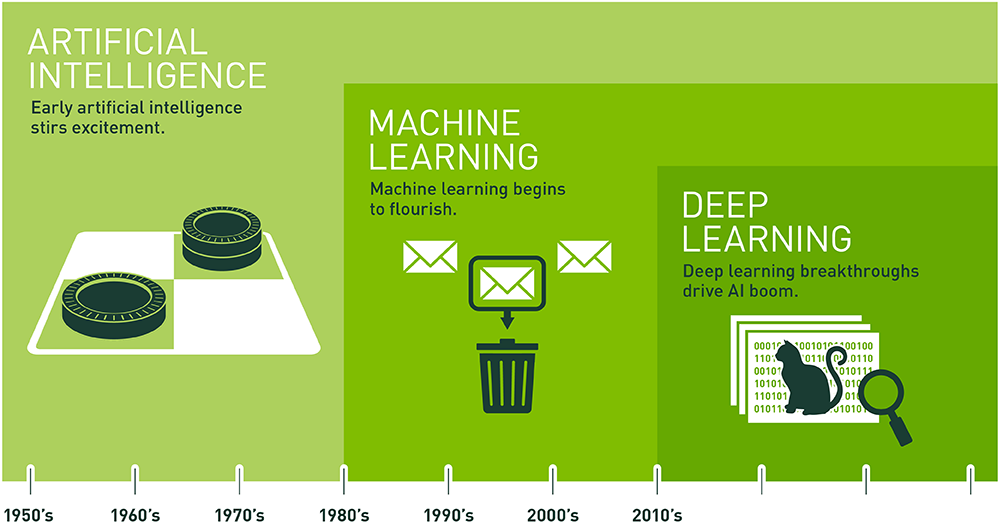
\includegraphics[totalheight=8cm]{Images/history.png}
    \caption{Minh họa AI, ML và DL\cite{basicai}}
    \label{history}
\end{figure}

\subsection{Giải thuật Perceptron Learning Algorithm(PLA)}
\begin{itemize}
\item PLA là nền móng đầu tiên của DL, nó được ra đời vào năm 1957 bởi Frank Rosenblatt giải bài toán về phân lớp nhị phân. Vì nó là nền móng nên hiểu được cách hoạt động của giải thuật này sẽ hiểu được cơ bản về DL. Vì sau này khi phát triển lên người ta chỉ cả tiến nó chứ không phải thay thế.
\item Yêu cầu của bài toán đặt ra là tìm phương trình một đường thẳng phân hai lớp đã được gán nhãn nằm về hai phía của đường thẳng đó, gọi là class 1 và class 2. Ý tưởng cơ bản của PLA là dự đoán, xây hàm mất mát, dựa vào hàm mất mát để đánh giá dự đoán và cập nhật lại dự đoán mới khi nào tốt thì dừng lại.
\item Trong không gian n chiều gọi \textbf{x} = [$x_{1}$, $x_{2}$, ..., $x_{n}$] là tập hợp các điểm dữ liệu, mỗi điểm được biểu diễn bằng một vector n chiều. \textbf{y} = [$y_{1}$, $y_{2}$, ..., $y_{n}$] là nhãn tức là giá trị lớp của mỗi điểm trong \textbf{x} tương ứng, $y_{i}$ = 1 nếu $x_{i}$ thuộc class 1, $y_{i}$ = -1 nếu $x_{i}$ thuộc class 2.
\item Ta giả sử đường thẳng cần tìm có phương trình:\[f_{x}(x) = w_{1}x_{1}+...+w_{n}x_{n}+w_{0}=w^{T}x = 0\]
Công việc của chúng ta là đi tìm các giá trị $w_{i}$ này hay còn gọi là các trọng số (weights).
\item Để dễ hình dung khi đi vào tính toán, ta sẽ đi tiếp trong trường hợp là không gian hai chiều (các công thức vẫn viết tổng quát cho n chiều). Ta giả sử đường thẳng $w_{1}$$x_{1}$ + $w_{2}$$x_{2}$ + $w_{0}$ = 0 là nghiệm của bài toán. Khi đó với điểm x chưa có nhãn, ta có thể gán nhãn cho nó bằng cách  \[label(x) = 1 \quad if \quad w^T \geq 0, \quad else \quad -1\] hay ngắn gọn là label(x) = sgn($w^{T}x$) với sgn là hàm xác định dấu.
\item Hàm mất mát này tính dựa trên số điểm bị phân lớp sai. Với mỗi điểm phân lớp sai thì y và $w^{T}$$x_{i}$ trái dấu, và khi phân lớp sai khoảng cách của điểm đó càng lớn thì giá trị hàm lỗi càng tăng. Việc chúng ta cần làm là đi tối ưu hàm lỗi này từ đó cập nhật được trọng số $w$. Ở đây sẽ đề xuất một phương pháp tối ưu áp dụng Gradient Descent đó là xét mỗi điểm bị phân lớp sai, khi đó giá trị mất mát cho điểm đó là: \[J(w; x_i; y_i) = -y_i w^T x_i\] có đạo hàm là $\Delta _{w}$J(w; $x_{i}$; $y_{i}$) = -$y_{i}$$x_{i}$.
\item Ta có quy tắc cập nhật là: $w_{t+1}^{T}$$x_{i}$ = ($w_{t}+y_{i} x_{i} )^{T}$$x_{i}$ =  $w_{t}^{T}$$x_{i}$ + $y_{i}$ $\left \| x_i \right \| ^{2}$.
Nhận thấy khi $w_{t}^T$$x_{i}$ và $y_{i}$ trái dấu, khi cập nhật lại thì $w_{t+1}^Tx_{i}$ < $w_{t}x_{i}$ nên hàm lỗi sẽ nhỏ đi theo mỗi bước cập nhật. Kết quả cuối cùng sẽ tối ưu nếu tập input có dạng tuyến tính. Mô hình minh họa cho PLA như Hình \ref{pla}. 
\end{itemize}

\begin{figure}[ht]
\centering
        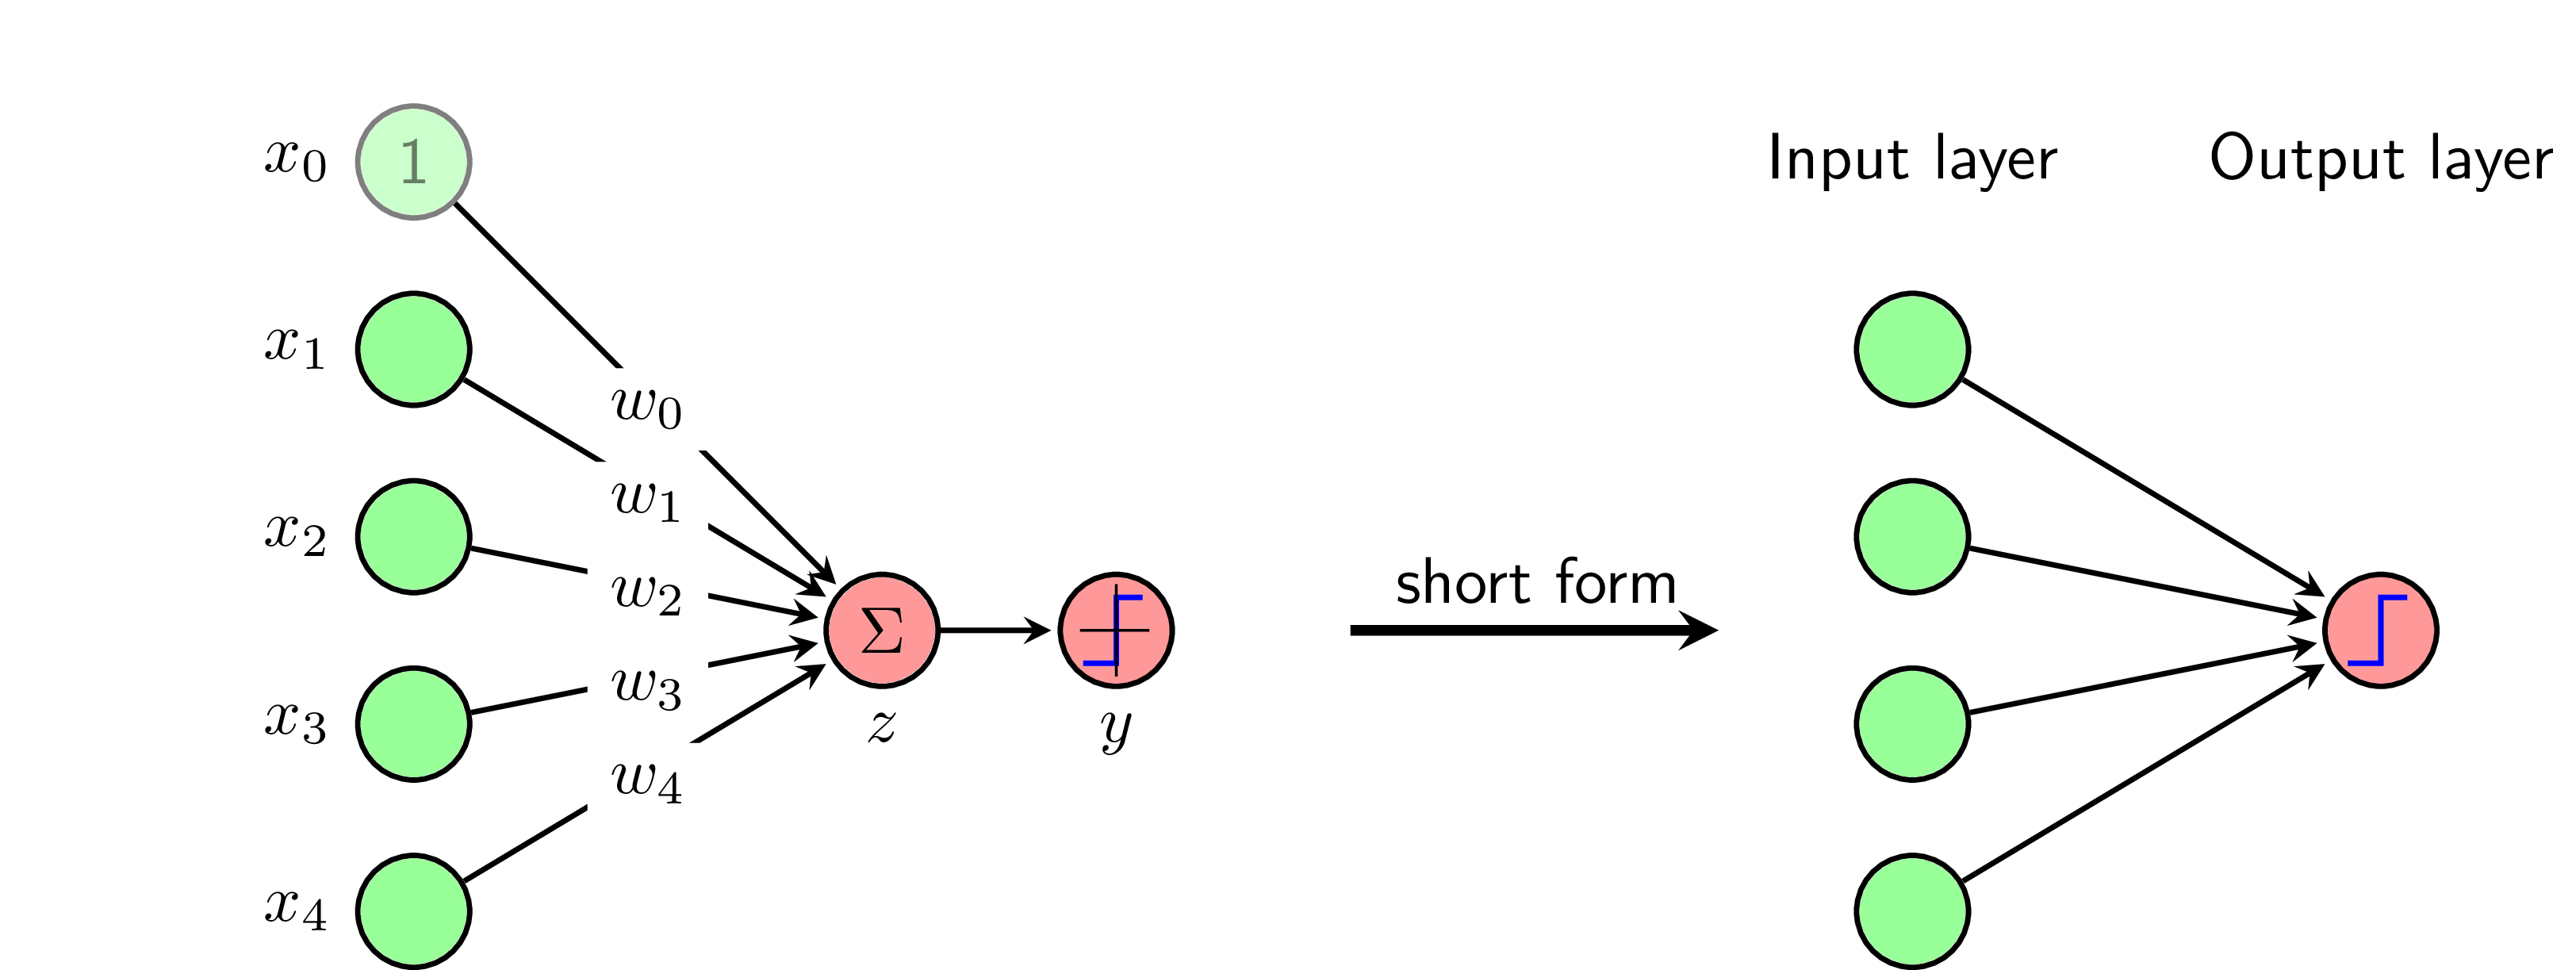
\includegraphics[totalheight=5cm]{Images/first_ann.png}
    \caption{Mô hình nơ-ron cho PLA \cite{basicdeep}}
    \label{pla}
\end{figure}

\begin{itemize}
\item Qua đây ta có thể giải thích được một số thành phần cơ bản trong một mạng nơ-ron. Lớp input là các giá trị $x$, các giá trị $w$ là các trọng số(weights), giá trị $x_{0}$=1 sau này sẽ được gọi là bias.
\item Với $z = w^{T}x$, ta có $y=sgn(z)$ là output của mạng. Hàm $sgn()$ được gọi là activation function.
Còn hàm lỗi thì chúng ta tự xây dựng và tự tối ưu miễn sao giải thuật có hiệu quả.
\end{itemize}
\subsection{MLP và Backpropagation}
\begin{itemize}
\item Mặc dù PLA mang lại nhiều triển vọng lúc mới ra đời nhưng về bản chất thì nó không thể giải quyết được với tập dữ liệu phi tuyến và nó được chứng minh trong cuốn sách Perceptrons, điều này làm cho giải thuật này không phát triển được thêm trong hai mươi năm. Thời kỳ này còn được gọi là mùa đông AI thứ nhất(The first AI winter).
\item Mãi tới năm 1986, Geoffrey Hinton cùng cộng sự viết một bài báo có tên Learning representations by back propagating error chứng minh được rằng mạng nơ-ron với nhiều lớp ở giữa(gọi là hidden layer) có thể biểu diễn được các quan hệ phi tuyến với quy trình gọi là backpropagation và sau mỗi lớp là một hàm kích hoạt phi tuyến sigmoid hoặc tanh. Lúc này nó được gọi là Multi-layer Perceptron(MLP).
\item MLP cải tiến thêm chỗ thay vì chỉ có hai lớp input và output như PLA thì nó sẽ có thêm nhiều hidden layer ở giữa. Mỗi node ở các lớp này gọi là một Unit, input của mỗi Unit sẽ là output của lớp trước đó qua activation function. Giá trị $z$ ở mỗi Unit sẽ cộng thêm một giá trị $b$ được gọi là bias. Với MLP thì giá trị $b$ này không cố định là $1$ mà nó sẽ thay đổi trong quá trình học, qua các lớp, trên từng Unit.
\item Backpropagation là một phương pháp sử dụng để tối ưu hàm lỗi cho MLP, nó giúp tính gradient ngược từ lớp cuối cùng đến lớp đầu tiên dựa vào cách tính đạo hàm của hàm hợp. Nhờ đây mà mạng nơ-ron tiếp tục được phát triển cho tới khoảng 1990 do gặp phải vấn đề tiếp theo.
\end{itemize}
\subsection{Mùa đông AI thứ hai và sự ra đời của mạng học sâu}
\begin{itemize}
\item Vấn đề phi tuyến đã được giải quyết nhưng việc tối ưu hàm lỗi của mạng nơ-ron quá phức tạp khi gặp bài toán khó và dữ liệu đầu vào lớn vì nó không phải là một hàm lồi. Tiếp đến là việc các hidden layer mở rộng làm cho khả năng tính toán mất quá nhiều chi phí, làm cho việc huấn luyện không hiệu quả, và hơn nữa là vấn đề vanishing gradient (gradient bỏ qua những thành phần có đạo hàm =0). Những hạn chế này làm cho mạng nơ-ron bị thay thế dần bởi một giải thuật mới có tên là Support Vector Machine(SVM) trong giai đoạn 1990-2000. Giai đoạn này còn gọi là Mùa đông AI thứ hai.
\item Tới 2006, mạng nơ-ron được cải tiến bởi Hinton với khái niệm autoencoder. Ta có thể hiểu khái niệm nay bằng cách xây dựng nó như sau. Xây dựng một autoencoder là xây dựng một mạng nơ-ron chỉ có một hidden layer, số Unit của hidden layer này ít hơn số input và output thì bằng với input. Ta sẽ huấn luyện mạng này sao cho giá trị output giống với giá trị input. Vì mạng chỉ có một hidden layer nên ta có thể gọi giai đoạn từ input tới hidden layer là mã hóa, còn từ hidden layer tới output là giải mã. Quá trình này thành công, ta sẽ bỏ đi output vì về bản chất thì hidden layer tuy ít node hơn nhưng vẫn mang đầy đủ tính chất của input. Ta tiếp tục xây dựng một autoencoder từ hidden layer này và cứ thế cho đến khi đạt được một mạng đủ sâu mà output của mạng này mang được những đặc điểm của input. Sau đó ta tiếp tục làm việc với output này theo yêu cầu bài toán. Việc này sẽ làm giảm thiếu rất nhiều vấn đề vanishing gradient. Từ ý tưởng này, mạng nơ-ron được cộng đồng tiếp tục đón nhận và cũng kể từ đây cái tên mạng học sâu(Deep Learning) ra đời.
\item Năm 2012 là năm có nhiều biến động nhất, cũng kể từ đây mà DL chiếm ưu thế vượt trội hoàn toàn so với các phương pháp khác trong cùng lĩnh vực. Đầu tiên là việc ra đời của ReLU và dropout do Geoffrey Hinton và cộng sự công bố, hai kỹ thuật này khá đơn giản nhưng lại đem lại kết quả ngoài sức mong đợi. ReLU là hàm với output là 1 khi đầu vào không âm, là 0 khi ngược lại, còn dropout là trong quá trình huấn luyện một số hidden unit bị tắt ngẫu nhiên và khi test thì sẽ kích hoạt lại toàn bộ. Những phương pháp này mang lại nhiều hiệu quả và giảm thiểu được vanishing gradient. Tiếp đến là việc tận dụng được hiệu năng của GPU trong quá trình huấn luyện (GPU là card đồ họa với mục đích chính sản xuất là để chơi game với khả năng chạy song song nhiều lõi nhưng lại rất thích hợp khi huấn luyện các mạng học sâu, làm cho việc huấn luyện nhanh hơn rất nhiều lần).
\item Từ đó tới nay, mạng học sâu được sử dụng một cách rộng rãi hơn, các sản phẩm sử dụng nó, các nhà nghiên cứu, người học đều tăng cao, đồng thời các công cụ hỗ trợ việc code và huấn luyện cũng tăng lên nhanh chóng.
\end{itemize}

\section{Mạng nơ-ron học sâu tích chập và ứng dụng cho phân đoạn ảnh}

% Toàn bộ kiến trúc CNN được minh họa như Hình \ref{cnn}.

% \begin{figure}[ht]
% \centering
%         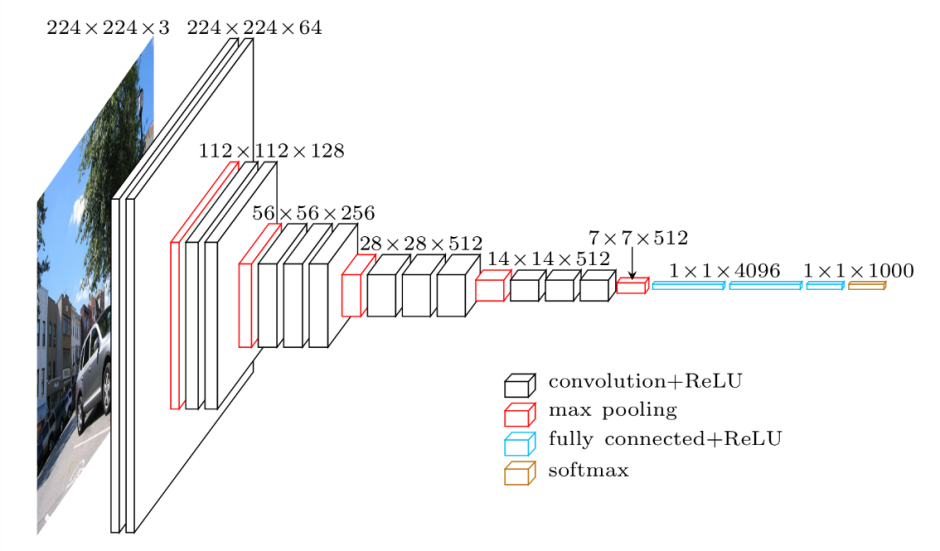
\includegraphics[totalheight=9cm]{Images/cnn.png}
%     \caption{Kiến trúc CNN\cite{accarchitect}}
%     \label{cnn}
% \end{figure}

\subsection{Lớp kết nối đầy đủ và vấn đề của nó}
Mục vừa rồi đã trình bày giải thuật cơ sở của phương pháp học sâu là PLA. Khi ta nhìn giải thuật này dưới mô hình mạng sẽ thấy mạng gồm hai lớp là đầu vào (input) gồm nhiều nút mạng và đầu ra (output) gồm một nút mạng. Nếu ta chèn thêm vào giữa hai lớp này một lớp mạng gồm nhiều nút nữa, và kết nối tất cả các nút mạng ở lớp này với tất cả các nút ở lớp sau và lớp trước cùng các trọng số (có thể tiếp tục thêm nhiều lớp khác nữa), ta sẽ được một mô hình học tri giác nhiều lớp (Multilayer Perceptron) và mỗi lớp trong đó được gọi là lớp kết nối đầy đủ. Đây chính là kiến trúc mạng nơ-ron truyền thống.\\
Các mạng nơ-ron truyền thống này được kỳ vọng có thể giải những bài toán phức tạp với độ chính xác cao nhưng vấn đề chi phí đôi khi lại làm cho nó trở nên không khả thi. Đặc biệt sử dụng nó trong lĩnh vực xử lý ảnh. Ta lấy ví dụ một ảnh đầu vào có kích thước dài 128, rộng là 128 , ba giá trị màu là RGB sẽ có ít nhất 128x128x3 = 49125 tham số cho lớp mạng đầu tiên để xử lý bức ảnh này, và để tránh lượng thông tin mất mát, số tham số của các lớp sau cũng sẽ tương đương lớp đầu. Điều này dẫn tới cần một sức mạnh tính toán cũng như bộ nhớ khổng lồ để giải quyết các bài toán xử lý ảnh. Một vấn đề khác mà các mạng nơ-ron phức tạp còn mắc phải vấn đề quá khớp (overfitting). Để giải quyết vấn đề này mạng, người ta bắt đầu sử dụng lớp tích chập thay thế cho các lớp đầy đủ. Mô hình sử dụng các lớp tích chập này chính là mạng nơ-ron tích chập (Convolutional Neural Networks hay ngắn gọn là CNN) là một dạng cải tiến của mạng nơ-ron nhân tạo được sử dụng. Ta sẽ đi vào phân tích một số đặc điểm của CNN để hiểu về rõ về cách giải quyết vấn đề của thiết kế mạng này.

\subsection{Lớp tích chập}
Trong xử lý ảnh và thị giác máy tính, người ta phân rõ hai khái niệm phép toán tích chập (convolution) và phép toán tương quan (correlation) qua điểm khác nhau duy nhất ở quá trình tính toán là đảo ngược ma trận lõi ở phép tích chập trước khi tính. Để dễ hình dung ta xem xét ví dụ sau đây với ma trận đầu vào 1-chiều $I$ (độ dài $i=9$) và lõi 1-chiều $K$ (độ dài $k=3$):
$$ I = [1, 2, 3, 4, 5, 6, 7, 8, 9]$$
$$ K = [2, 4, 6] $$
Thì kết quả của phép tính tương quan được tính như sau:
$$ Correlation(I,K)_{c = \overline{0, i - k - 1}} = \sum_{m=c}^{c + k-1}I_{m}*K_{m-c}$$
$$ Correlation(I,K) = [1*2 + 2*4 + 3*6, ... , 7*2 + 8*4 + 9*6] $$
$$ Correlation(I,K) = [28,  40,  52,  64,  76,  88, 100] $$
Và kết quả của phép tính tích chập được tính như sau:
$$ Convolution(I,K)_{c = \overline{0, i - k - 1}} = \sum_{m=c}^{c + k-1}I_{m}*K_{k - 1 - m + c}$$
$$ Convolution(I,K) = [1*6 + 2*4 + 3*2, ... , 7*6 + 8*4 + 9*2] $$
$$ Convolution(I,K) = [20, 32, 44, 56, 68, 80, 92] $$
Công thức trên tham khảo tại \cite{convSlide}. tương tự khi I, K là các ma trận 2, 3 chiều. Để dễ hình dung ta xem hình minh hoạ \ref{convExample}.

\begin{figure}[h]
\centering
    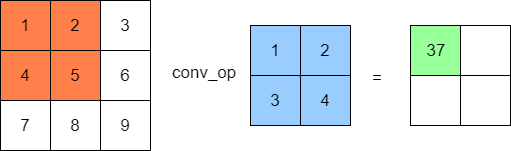
\includegraphics[totalheight=3cm]{Images/conv.png}
    \caption{Một phần quá trình tính tương quan trong xử lý ảnh}
    \label{convExample}
\end{figure}
Ta có thể thấy ở phép tính tương quan trên ma trận, tuỳ vào ma trận lõi $K$ mà ma trận kết quả sẽ có được một số tính chất đặt biệt, ví dụ ở hình \ref{convExample} ta sẽ nhận được ma trận kết quả làm nổi bật các cạnh dọc ở ma trận đầu vào. Điều tương tự cũng xảy ra với kết quả của phép tính tích chập vì hai phép tính này là gần giống nhau ở cách tính. Trong các phép tính xử lý ảnh, tuỳ vào tình huống mà người ta sử dụng phép tích chập hoặc phép tính tương quan để nhầm đạt được độ lợi về thời gian tính toán khi tính áp dụng các tính chất kết hợp lên một dãy các phép tính tích chập (tương quan) liên tục\cite{convtheorem}.\\
Tuy nhiên ở các mạng học sâu, phép tính tích chập được dùng để chỉ phép tính tương quan. Các nên tảng học sâu được hỗ trợ như Tensorflow sử dụng từ khoá tích chập và lớp tích chập để chỉ phép tính tương quan trong xử lý ảnh. Vì như đã nói ý nghĩa của hai phép tính này là như nhau, tuỳ vào độ lợi tính toán mà người ta sẽ quyết định sử dụng phép tính nào.\\
Khi sử dụng lớp tích chập thay cho lớp kết nối đầy đủ ở mạng học sâu sẽ có một số khác biệt sau:
\begin{itemize}
    \item Bộ nhớ tính toán sử dụng các lớp tích chập sẽ nhỏ hơn.
    \item Thời gian tính toán khi sử dụng các lớp tích chập sẽ nhanh hơn.
    \item Ở những lớp càng sâu, một điểm dữ liệu khi sử dụng các lớp tích chập sẽ bị ảnh hưởng bới nhiều điểm dữ liệu đầu vào hơn thay vì là như nhau ở tất cả các lớp.
\end{itemize} 
Trong mạng học sâu, quá trình học sẽ giúp cập nhật các trọng số của ma trận lõi $K$ ở lớp tích chập này.

\subsection{Lớp gộp}
Lớp gộp (pooling), đôi khi được gọi là lớp giảm kích thước mẫu (sub-sampling), thường được sử dụng sau một số lớp tích chập nhất định. Vì người ta thấy rằng nếu dữ nguyên kích thước của ảnh sẽ tạo ra một số rất lớn trọng số làm cho mạng phải tính toán nhiều hơn và khó huấn luyện hơn do hiện tượng quá khớp (overfitting). Lớp gộp này đóng vai trò làm giảm kích thước ảnh nhưng vẫn đảm bảo giữ lại các dữ liệu cần thiết nhằm qua đó làm giảm số lượng phép tính toán và tránh tình trạng quá khớp vừa nêu.\\
Lớp gộp có thể sử dụng nhiều loại hàm gộp khác nhau như hàm trung bình hoặc hàm lấy lớn nhất (phổ biến) tuỳ thuộc vào đặc điểm của bài toán. Các lớp gộp này thường có kích thước bằng với độ cách (stride), tức là chúng sẽ có ý nghĩa như một phép thay thế một vùng các điểm dữ liệu chỉ bằng một điểm dữ liệu duy nhất, và các vùng này không có điểm trùng.\\
Ta có thể thấy sau khi qua một lớp gộp, các vùng khác nhau sẽ nằm gần nhau hơn và nhờ vậy với lớp tính tích chập tiếp theo sẽ có được thông tin của một vùng lớn hơn ở ảnh ban đầu. Vì vậy sau khi qua càng nhiều lớp gộp, ảnh (đặc trưng) sẽ có ý nghĩa toàn cục hơn là ý nghĩa chi tiết. Đây cũng là một yếu điểm của lớp gộp cho bài toán phân đoạn ảnh mà không thay đổi kích thước của nó.\\
Trong quá trình học, lớp gộp không có các trọng số có thể học được.

\begin{figure}[h]
\centering
    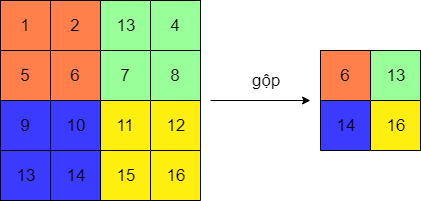
\includegraphics[totalheight=3.5cm]{Images/max-pool.png}
    \caption{Phép tính gộp lấy lớn nhất với kích thước 2, độ cách 2}
    \label{poolExample}
\end{figure}

\subsection{Lớp đảo tích chập}
Phép đảo tích chập, có tên gọi khác là phép chuyển vị (transpose), là phép tính ngược lại với phép tích chập. Ở phép đảo tích chập, mỗi giá trị trong ma trận ảnh gốc $S$ sẽ được nhân với một ma trận trọng số lõi $K$ để được một vùng giá trị của ảnh kết quả $R$, các vùng này có thể chồng lấn lên nhau tuỳ vào độ cách (stride) và kích thước của $K$. Trong xử lý ảnh, phép đảo tích chập thường được dùng để phóng to và làm rõ các loại ảnh như ảnh chụp kính hiển vi, ảnh nguyên tử, ảnh thiên văn...\\
Trong mạng học sâu, quá trình học sẽ giúp cập nhật các trọng số của ma trận lõi $K$ ở lớp đảo tích chập này.

\begin{figure}[h]
\centering
    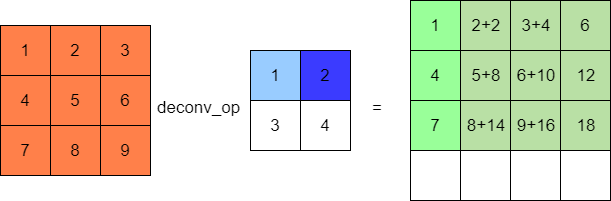
\includegraphics[totalheight=3.5cm]{Images/deconv.png}
    \caption{Một phần quá trình tính đảo tích chập với kích thước 2, độ cách 1}
    \label{deconvExample}
\end{figure}

\begin{figure}[h]
\centering
    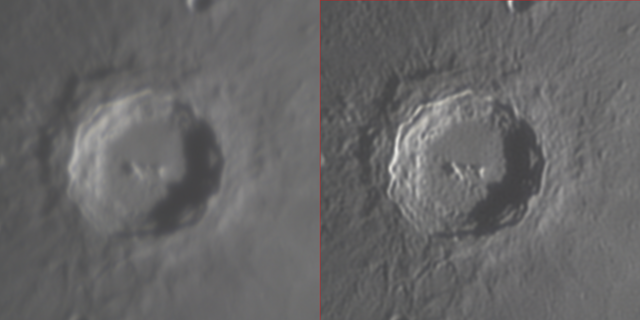
\includegraphics[totalheight=3.5cm]{Images/realConvEx.png}
    \caption{Ảnh chụp thiên văn trước và sau khi được xử lý đảo tích chập}
    \label{deconvRealExample}
\end{figure}

\subsection{Lớp đảo gộp}
Để tạo ra một bức ảnh có kích thước lớn hơn ảnh gốc, người ta có nhiều phương pháp khác nhau. Ví dụ có thể sử dụng các phương pháp như: dùng phép toán đảo tích chập với độ cách lớn hơn 1, dùng phép biến đổi tuyến tính để tạo ra giá trị của điểm ảnh ở giữa hai điểm ảnh kể nhau, lặp lại điểm ảnh tạo ra các điểm lân cận. Trong \cite{unpoolref}, các tác giả giới thiệu phép đảo gộp với bảng nhớ được thực hiện như sau: khi thực hiện phép gộp giữ lại vị trí của các giá trị được lấy, khi thực hiện phép đảo gộp hằng số dùng bảng vị trí đã nhớ để tái tạo lại vị trí có giá trị khác hằng số đã chọn.\\
Trong quá trình học, lớp đảo gộp không có các trọng số có thể học được.

\begin{figure}[h]
\centering
    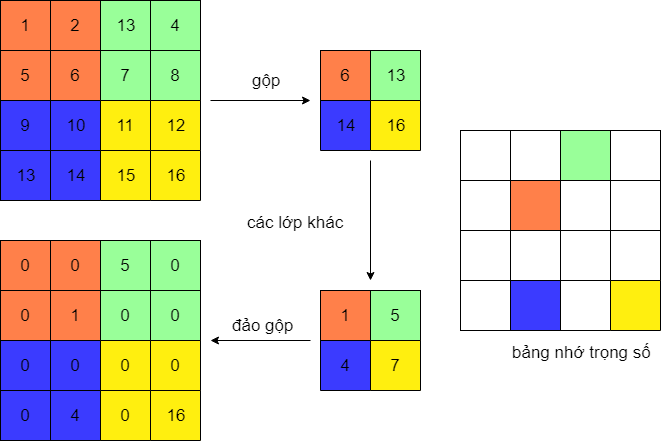
\includegraphics[totalheight=7.5cm]{Images/unpool.png}
    \caption{Minh hoạ phép đảo gộp với bảng nhớ}
    \label{unpoolExample}
\end{figure}

\subsection{Ứng dụng vào bài toán phân đoạn ảnh}
Như đã để cập, các mô hình mạng nơ-ron học sâu khi sử dụng cho xử lý ảnh sẽ gặp vấn đề quá tải số trọng số. Vì vậy các mạng học sâu sẽ sử dụng các lớp tích chập để giải quyết vấn đề này.\\
Tuy nhiên nếu chỉ sử dụng nhiều lớp tích chập liên tiếp nhau, vẫn có thể gây ra quá tải về trọng số nếu độ sâu của mạng đủ lớn. Nếu như giảm độ sâu của mạng thì các đặc điểm mang tính phổ quát của ảnh sẽ không được học. Vì vậy lớp gộp được sử dụng sau một số lớp tích chập nhất định để nhằm giảm đi số trọng số của mạng mà vẫn đảm bảo được chiều sâu cần có để mạng có thể học được các thông tin phổ quát.\\
Khi đặt vào bài toán phân đoạn ảnh, rõ ràng sau khi đi qua một số các lớp gộp, kích thước ảnh đã được thay đổi và nhỏ hơn kích thước ban đầu. Để tái tạo lại kích thước này người ta thường sử dụng các lớp mạng làm tăng kích thước như đảo tích chập với độ cách lớn hơn một hoặc sử dụng lớp đảo gộp kết hợp với lớp tích chập hoặc kết hợp lớp đảo gộp với lớp đảo tích chập...\\
Ví dụ mạng Unet sử dụng phép lặp lại điểm ảnh, phép tích chập và phép cộng theo số kênh trong quá trình tái tạo lại kích thước ban đầu của ảnh.

% \begin{figure}[h]
% \centering
%     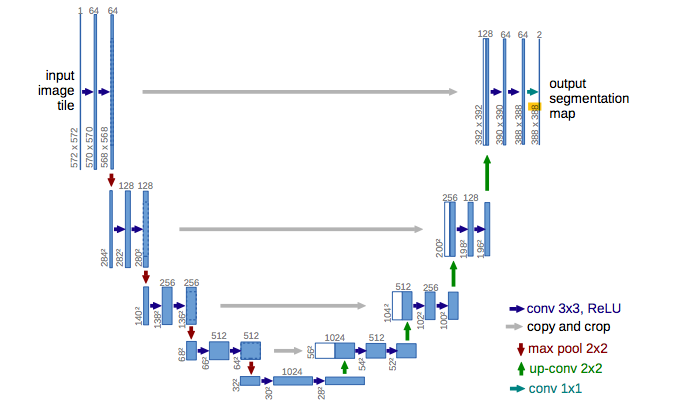
\includegraphics[totalheight=9.5cm]{Images/unet.png}
%     \caption{Kiến trúc mạng Unet}
%     \label{unetPic}
% \end{figure}

\section{Kỹ thuật lan toả bất đẳng hướng}
(Tên gọi trong tiếng Anh của kỹ thuật này là Anisotropic diffusion.)
Như đã nói nếu ta sử dụng phép toán tích chập của một ảnh với một ma trận phù hợp sẽ được một ảnh gồm các cạnh của ảnh gốc. Ta xem xét ứng dụng chúng vào ảnh \ref{fig:ww2} chụp một sân bay để nhận diện cạnh chính. Ảnh này đủ rõ để một người bình thường có thể nhận diện ra các đường băng của sân bay, các cạnh khối của toà nhà. Khi chú ý kỹ ta có thể thấy các chi tiết bề mặt như đường băng, toà nhà không mượt và có các đường nét nhỏ nằm ở trên đó. Vì vậy khi sử dụng một ma trận lõi nhận diện cạnh trực tiếp như ma trận sobel ta sẽ được một kết quả gồm nhiều cạnh nhiễu (không mong muốn) kèm với những cạnh thực như hình \ref{fig:ww2_sobel}; \\

\begin{figure*}
  \centering
  \subfigure[Ảnh gốc]{%
    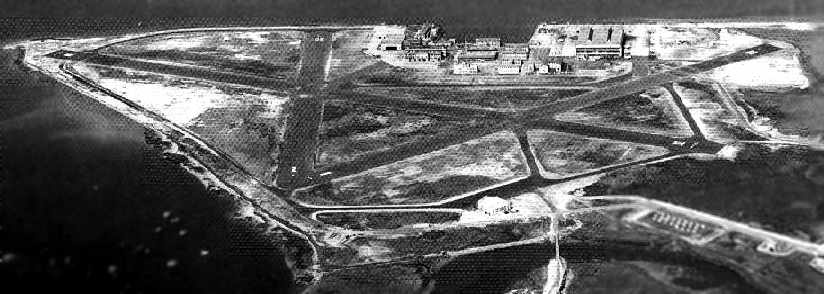
\includegraphics[width=0.75\textwidth]{Images/ww2.jpg}%
    \label{fig:ww2}%
    }
    \subfigure[Kết quả tích chập với ma trận nhận diện cạnh]{%
    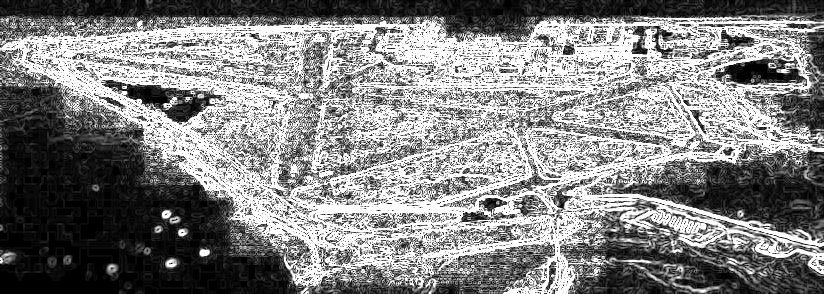
\includegraphics[width=0.75\textwidth]{Images/ww2_sobel.jpg}%
    \label{fig:ww2_sobel}%
    }
  \caption{Minh hoạ sử dụng phép tích chập lấy cạnh trực tiếp}
  \label{fig:simplesobel}
\end{figure*}

Ví dụ một ma trận sobel có thể sử dụng:
$$\begin{bmatrix}
-1 & 0 & 1\\ 
-2 & 0 & 2\\ 
-1 & 0 & 1
\end{bmatrix}$$

Để loại bỏ các cạnh không mong muốn trên, người ta sử dụng một phép tích chập khác trước khi sử dụng phép tích chập với sobel. Phép tích chập trung gian này thường được dùng với một ma trận lọc Gauss. \\
Ví dụ một ma trận Gauss có thể sử dụng:
$$\begin{bmatrix}
1 & 2 & 1\\ 
2 & 4 & 2\\ 
1 & 2 & 1
\end{bmatrix}$$
Sử dụng một ma trận Gauss như trên là một phép biến đổi đẳng hướng và tương tự với sử dụng một phép cập nhật khử nhiểu thoả: $\partial I(x,y,t)/\partial t = div(\nabla I)$ với $x, y$ là toạ độ của điểm ảnh, $t$ là thời gian biến đổi, $\nabla I$ là gradient của ảnh $I$.\\

\begin{figure*}
  \centering
  \subfigure[Ảnh sau khi khử nhiễu]{%
    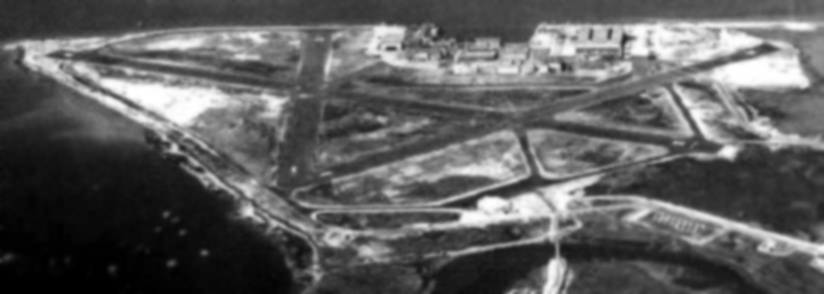
\includegraphics[width=0.75\textwidth]{Images/ww2_gauss.jpg}%
    \label{fig:ww2}%
    }
    \subfigure[Kết quả tích chập ảnh đã khử nhiễu đẳng hướng với ma trận nhận diện cạnh]{%
    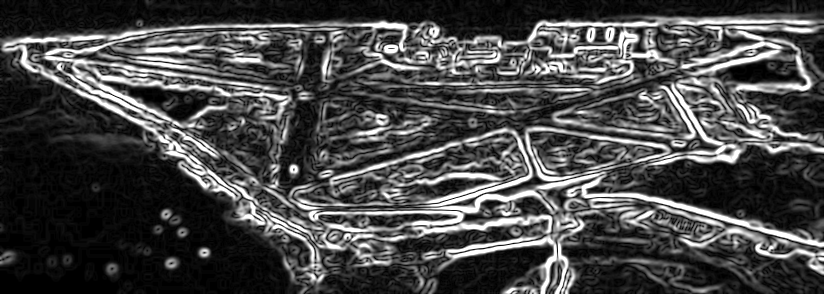
\includegraphics[width=0.75\textwidth]{Images/ww2_gauss_sobel.jpg}%
    \label{fig:ww2_sobel}%
    }
  \caption{Minh hoạ sử dụng phép tích chập lấy cạnh đã qua bước trung gian khử nhiễu Gauss}
  \label{fig:gausssobel}
\end{figure*}

Mặc dù đã loại bỏ được rất nhiều cạnh không cần thiết nhưng các cạnh bây giờ lại có hiện tượng bị nhoè và không còn chính xác vị trí cạnh nữa. Để giải quyết vấn đề này, Perona và Malik trong \cite{56205} đã đề xuất một cách cập nhật mới thoả: $\partial I(x,y,t)/\partial t = div(g(||\nabla||) \nabla I)$ với $g(||\nabla||)$ có khả năng tìm được vị trí các cạnh chính. Biến đổi công thức do Perna và Malik đề xuất trên về dạng rời rạc khi xử lý các điểm ảnh ta được công thức cập nhật:
$$I^{t+1}_{s} = I^{t}_{s} + \frac{\lambda }{\eta_{s}}\sum_{p \in \eta_{s}}g(\nabla I_{s,p})\nabla I_{s,p}.$$
Với một số kí hiệu mới $I^{t}_{s}$ là một điểm ảnh có toạ độ $s$ sau lần cập nhật $t$, $\eta_{s}$ là tập các điểm ảnh lân cận của điểm có toạ độ $s$, $\nabla I_{s,p}$ là gradient của điểm ảnh $I_{s,p}$, $\lambda$ là một hệ số cập nhật. Trong đó:
$$\nabla I_{p,s} = I_{p} - I_{s}^{t},$$
$g(x)$ có nhiều sự lựa chọn, ví dụ:
$$g(x) = \frac{1}{1 + {x^{2}/k}}.$$
Ta có thể thấy ở công thức mới này vai trò của các điểm ảnh lân cận khi cập nhật một điểm ảnh mới không còn chỉ phụ thuộc vào vị trí tương đối của nó với điểm cập nhật nữa. Vai trò của mỗi điểm lân cận này giờ còn phải phụ thuộc vào vị trí và giá trị của điểm ảnh được cập nhật.

% \begin{figure}
% \centering
%     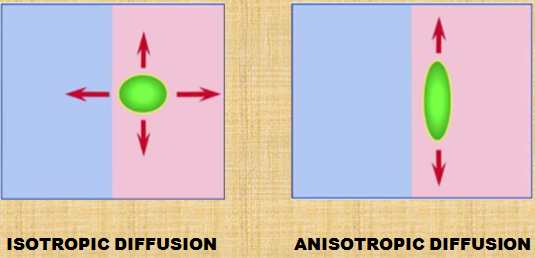
\includegraphics[totalheight=6cm]{Images/iso_aniso.png}
%     \caption{Minh hoạ cho phép biến đổi đẳng hướng và bất đẳng hướng}
%     \label{iso_aniso}
% \end{figure}

\begin{figure*}
  \centering
  \subfigure[Kết quả tích chập ảnh đã khử nhiễu đẳng hướng với ma trận nhận diện cạnh]{%
    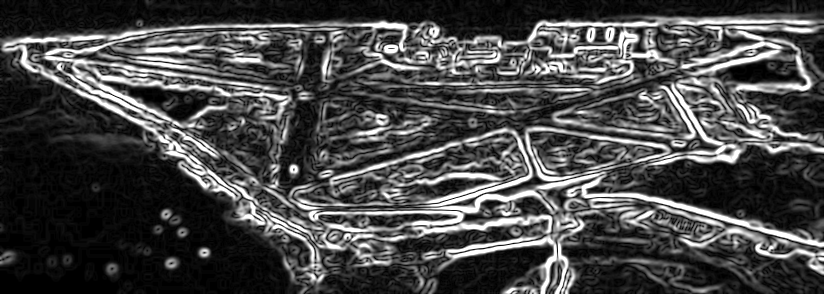
\includegraphics[width=0.75\textwidth]{Images/ww2_gauss_sobel.jpg}%
    \label{fig:ww2}%
    }
    \subfigure[Kết quả tích chập ảnh đã khử nhiễu bất đẳng hướng với ma trận nhận diện cạnh]{%
    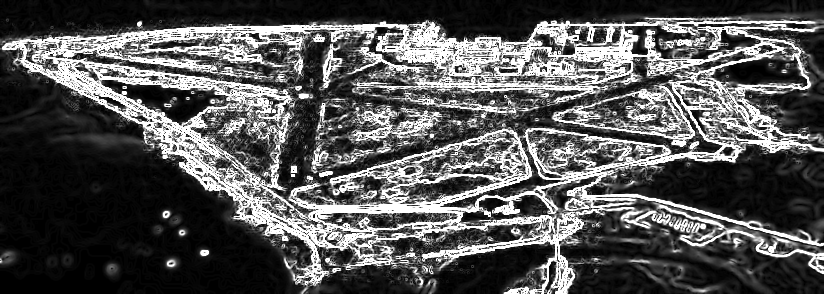
\includegraphics[width=0.75\textwidth]{Images/ww2_aniso_sobel.jpg}%
    \label{fig:ww2_sobel}%
    }
  \caption{So sánh sử dụng khử nhiểu trung gian đẳng hướng và bất đẳng hướng trước khi nhận diện cạnh}
  \label{fig:iso_aniso}
\end{figure*}

Nội dung và công thức trong mục này tham khảo tại \cite{661192} và \cite{56205}.


\section{Các chỉ số đánh giá kết quả phân đoạn}
Kết quả phân đoạn có thể được đánh giá bằng nhiều cách khác nhau. Đối với một bài toán nhất định, mỗi chỉ số đánh giá được lựa chọn cần phải nhạy cảm với một số đặc điểm phụ thuộc vào mục đích bài toán đó. Nếu bài toán để xác định thể tích vật thể, sai khác thể tích sẽ là chỉ số tiên quyết cho bài toán đó. Tuy nhiên với một kết quả phân đoạn cho ra thể tích chính xác hoàn toàn trên lý thuyết vẫn có thể bị sai hoàn toàn nếu như sử dụng chỉ số trùng giao trên hợp của voxel. Vì vậy, mỗi bài toán phải luôn dùng nhiều chỉ số phân đoạn khác nhau để đánh giá các giải pháp cho bài toán đó.\\
Trong luận văn này, chúng tôi sử dụng các chỉ số của cuộc thi phân đoạn lá gan trên tập dữ liệu SLiver07 và tập dữ liệu LiTS tham khảo tại \cite{SLiver07metric} và \cite{website:LiTS}. \\
Các chỉ số được chúng tôi sử dụng bao gồm:
\begin{itemize}
    \item \textbf{[Sliver07 - LiTS]} Chỉ số lỗi trùng thể tích (Volumetric overlap error - VOE), giá trị phần trăm. Chỉ số này được tính như sau: lấy tổng số voxel giao giữa dự đoán và nhãn chia cho tổng số voxel hợp giữa dự đoán và nhãn, lấy 1 trừ kết quả đó rồi nhân cho 100.
    \item \textbf{[Sliver07 - LiTS]} Chỉ số sai khác thể tích (Relative volume difference - VD hay RVD), giá trị phần trăm. Chỉ số này được tính bằng hiệu số số voxel của dự đoán và nhãn, chia cho  số voxel của nhãn, nhân 100. Chỉ số này nhận giá trị âm khi thể tích phân đoạn nhỏ hơn thể tích nhãn và nhận giá trị dương khi thể tích phân đoạn lớn hơn thể tích nhãn. Khi sử dụng cho tính điểm trong hệ thống của Sliver07, chỉ số này sẽ được lấy giá trị tuyệt đối(Relative absolute volume difference).
    \item \textbf{[Sliver07 - LiTS]} Khoảng cách mặt đối xứng trung bình (Average symmetric surface distance - AvgD), giá trị milimet. Voxel cạnh của vật thể là voxel có ít nhất 1 trong 18 láng giềng không thuộc vật thể. Khoảng cách mỗi voxel tới bề mặt là khoảng cách ngắn nhất từ voxel đó đến một voxel thuộc bề mặt. Khoảng cách trung bình giữa hai bề mặt là giá trị trung bình của tất cả các voxel tới bề mặt kia (voxel thuộc dự đoán tới bề mặt nhãn, voxel thuộc nhãn tới bề mặt dự đoán).
    \item \textbf{[Sliver07]} Khoảng cách mặt đối xứng bình phương từ gốc (Root Mean Square symmetric surface distance - RMSD), giá trị milimet. Giá trị này được tính giống với  AvgD nhưng khoảng cách ban đầu sẽ được bình phương lên và lấy trung bình.
    \item \textbf{[Sliver07 - LiTS]} Khoảng cách mặt lớn nhất (Maximum symmetric surface distance - MaxD), giá trị milimet. Chỉ số này tính giống AD nhưng thay vì lưu trung bình sẽ lưu giá trị lớn nhất.
    \item \textbf{[LiTS]} Chỉ số kẻ vuông (Dice), giá trị phần trăm. Chỉ số này đánh giá mức độ trùng của kết quả phân đoạn so với phép phân đoạn thật.
\end{itemize}
Các chỉ số từ cuộc thi Sliver07 sẽ được tính ra điểm cho từng chỉ số và cuối cùng tính trung bình ra tổng điểm cho một kết quả phân đoạn. Với mỗi chỉ số, mức điểm hoàn hảo là 100 điểm, mức điểm chấp nhận được là 75 điểm, mức điểm thấp nhất là 0 điểm. Mức điểm hoàn hảo là kết quả phân đoạn của chuyên gia đã có kinh nghiệm cho lĩnh vực phân đoạn bộ phận đó. Mức điểm chấp nhận được là của sinh viên y khoa chưa có kinh nghiệm phân đoạn khi so với kết quả của chuyên gia. Các chỉ số này là các chỉ số lỗi, càng thấp tức là kết quả phân đoạn càng tốt. Điểm cho mỗi chỉ số sẽ bằng 100 trừ đi chỉ số nhân với một hệ số đã xác định, và lấy lớn hơn với 0. \\
Trong cuộc thi LiTS các chỉ số không được quy ra điểm, thứ hạng của các nhóm tham dự sẽ dựa vào chỉ số Dice Score trung bình trên tất cả ảnh 3-chiều.

\begin{table}
\begin{center}
\begin{tabular}{ |l|c| } 
\hline
\Gape[0.1cm][0.1cm]{Tên chỉ số} & Công thức chỉ số \\ 
\hline
\textbf{VOE} &\Gape[0.5cm][0.5cm]{$(1 - {R \bigcap G}/{R\bigcup G})*100\%$ }\\ 
\hline
\textbf{VD} & \Gape[0.5cm][0.5cm]{$(|R| -|G|)/|G|*100\%$} \\ 
\hline
\textbf{AvgD} & \Gape[0.5cm][0.5cm]{$(\sum d(S(G),S(R)) + \sum d(S(R),S(G)))/(|S| + |G|)$}\\
\hline
\textbf{RMSD} & \Gape[0.5cm][0.5cm]{$\sqrt{(\sum d(S(G),S(R))^{2} + \sum d(S(R),S(G))^{2})/(|S| + |G|)}$} \\ 
\hline
\textbf{MaxD} & \Gape[0.5cm][0.5cm]{$max(max(d(S(G),S(R))), max(d(S(G),S(R))))$} \\ 
\hline
\textbf{Dice} & \Gape[0.5cm][0.5cm]{$2*{R \bigcap G}/(|R| + |G|)*100\%$ }\\ 
\hline
\end{tabular}
\caption{\label{tab:table-name1}Cách tính các chỉ số.}
\end{center}
\end{table}


\begin{table}[H]
\begin{center}
\begin{tabular}{ |l|c| } 
\hline
\Gape[0.1cm][0.1cm]{Tên chỉ số} & Công thức điểm \\ 
\hline
\textbf{VOE} & \Gape[0.5cm][0.5cm]{$100 - 100*\textbf{VOE}*25/6.4$} \\ 
\hline
\textbf{VD} & \Gape[0.5cm][0.5cm]{$100 - 100*\textbf{|VD|}*25/4.7$} \\ 
\hline
\textbf{AvgD} & \Gape[0.5cm][0.5cm]{$100 - 100*\textbf{AvgD}*25$} \\
\hline
\textbf{RMSD} & \Gape[0.5cm][0.5cm]{$100 - 100*\textbf{RMSD}*25/1.8$} \\ 
\hline
\textbf{MaxD} &\Gape[0.5cm][0.5cm]{ $100 - 100*\textbf{MaxD}*25/4.7$} \\ 
\hline
\end{tabular}
\caption{\label{tab:table-name}Cách tính điểm cho các chỉ số.}
\end{center}
\end{table}
 
Ý nghĩa của các ký hiệu như sau:
\begin{itemize}
    \item $G$: vật thể nhãn
    \item $R$: vật thể được dựa đoán bởi mô hình
    \item $\bigcap$: phần thể tích giao của hai vật thể
    \item $\bigcup$: phần thể tích hợp của hai vật thể
    \item $|R|$: tổng số voxel của vật thể R
    \item $S(R)$: bề mặt vật thể R
    \item $d(x,S(R))$: khoảng cách từ voxel x đến bề mặt vật thể R
    \item $d(S(G),S(R))$: khoảng cách một chiều từ bề mặt vật thể G tới bề mặt vật thể R, đây là tập hợp $\{ d(v_{0}, S(R)), d(v_{1}, S(R)),...d(v_{n}, S(R)) \} $ với $v \in S(G) $
    \item $\textbf{|VD|}$: giá trị tuyệt đối của chỉ số VD.
\end{itemize}

\section{Công nghệ sử dụng}
\subsection{Nền tảng Tensorflow}